\begin{center}
    \textbf{Алгебра}
\end{center} 


\samerowans{\begin{problem}{1}
Сравните значения выражений $A=\dfrac{50^3}{(2^2)^3 \cdot 5^6}$ и \\
$B=\dfrac{3^{32} - 3 \cdot 9^{14}}{26 \cdot 27^{10}}$.
В ответе запишите название меньшего.
\end{problem}}

\smallskip

\samerowans{\begin{problem}{2а}
Решите уравнение: $\dfrac{3x + 11}{2} - \dfrac{2x + 7}{3} = 4x$
\end{problem}}

\smallskip

\samerowans{\begin{problem}{2б}
Решите уравнение: $(2x + 1)^2 - 3(x - 5)^2 = (x + 3)(x - 3)$
\end{problem}}

\smallskip

\begin{problem}{2в}
Решите уравнение: $\bigl|\,|x+4|-2\,\bigr|=3$
\end{problem}

\smallskip

\noindent\grid{34}{12}

\smallskip

\begin{problem}{3}
Разложите на неразложимые множители (так, чтобы дальнейшее разложение было невозможно):
\end{problem}

\bigskip

\noindent \textbf{3а.} $-9c^2 + 12cd^2 - 4d^4$

\smallskip

\rowans{1ex}

\bigskip

\noindent \textbf{3б.} $x^2 + 8x + 16 - 9a^2$

\smallskip

\rowans{1ex}

\bigskip

\noindent \textbf{3в.} $27a^3c - 27a^2bc + 9ab^2c - b^3c$

\smallskip

\rowans{1ex}

\smallskip

\samerowans{\begin{problem}{4}
Моторная лодка плыла 4~часа по течению реки и 6~часов против течения, пройдя за это время 114~км. Найдите собственную скорость лодки, если скорость течения реки 3~км/ч.
\end{problem}}

\bigskip

\begin{problem}{5} Выполните задания. Условие для трёх пунктов --- общие:

\noindent \textbf{5а.}~Напишите уравнение прямой, если известно, что она проходит через точку $M(-3;\;2)$ и параллельна прямой, заданной уравнением $y = 4x$.

\noindent \textbf{5б.}~Найдите координаты точки пересечения этой прямой с прямой $y=-2x+20$.

\noindent \textbf{5в.}~Найдите координаты точки на прямой из пункта~а), абсцисса которой равна ординате.
\end{problem}

\noindent\grid{34}{18}

\begin{center}
\textbf{Геометрия}
\end{center}

\samerowans{\begin{problem}{6}
Угол, равный $150°$, разделён лучами, исходящими из вершины, на 5~равных углов. Сколько прямых углов при этом образовалось?
\end{problem}}

\smallskip

\samerowans{\begin{problem}{7}
В прямоугольном треугольнике биссектриса наибольшего угла пересекает гипотенузу под углом $80°$. Найдите острые углы данного треугольника.
\end{problem}}

\smallskip

\samerowans{\begin{problem}{8}
Найдите третью сторону равнобедренного треугольника, если две его стороны равны 10~см и 5~см.
\end{problem}}

\smallskip

\begin{problem}{9}
В прямоугольном треугольнике $ABC$ угол~$C$ прямой, внешний угол при вершине~$B$ равен $150°$, биссектриса~$AA_1$ равна 20~см. Найдите~$AC$.
\end{problem}

\noindent\grid{34}{18}

\smallskip

\begin{problem}{10}
На рисунке $AB \| CD$, $AB = CD$ и $AE = CF$. Докажите, что $BE \| DF$.

\smallskip

\noindent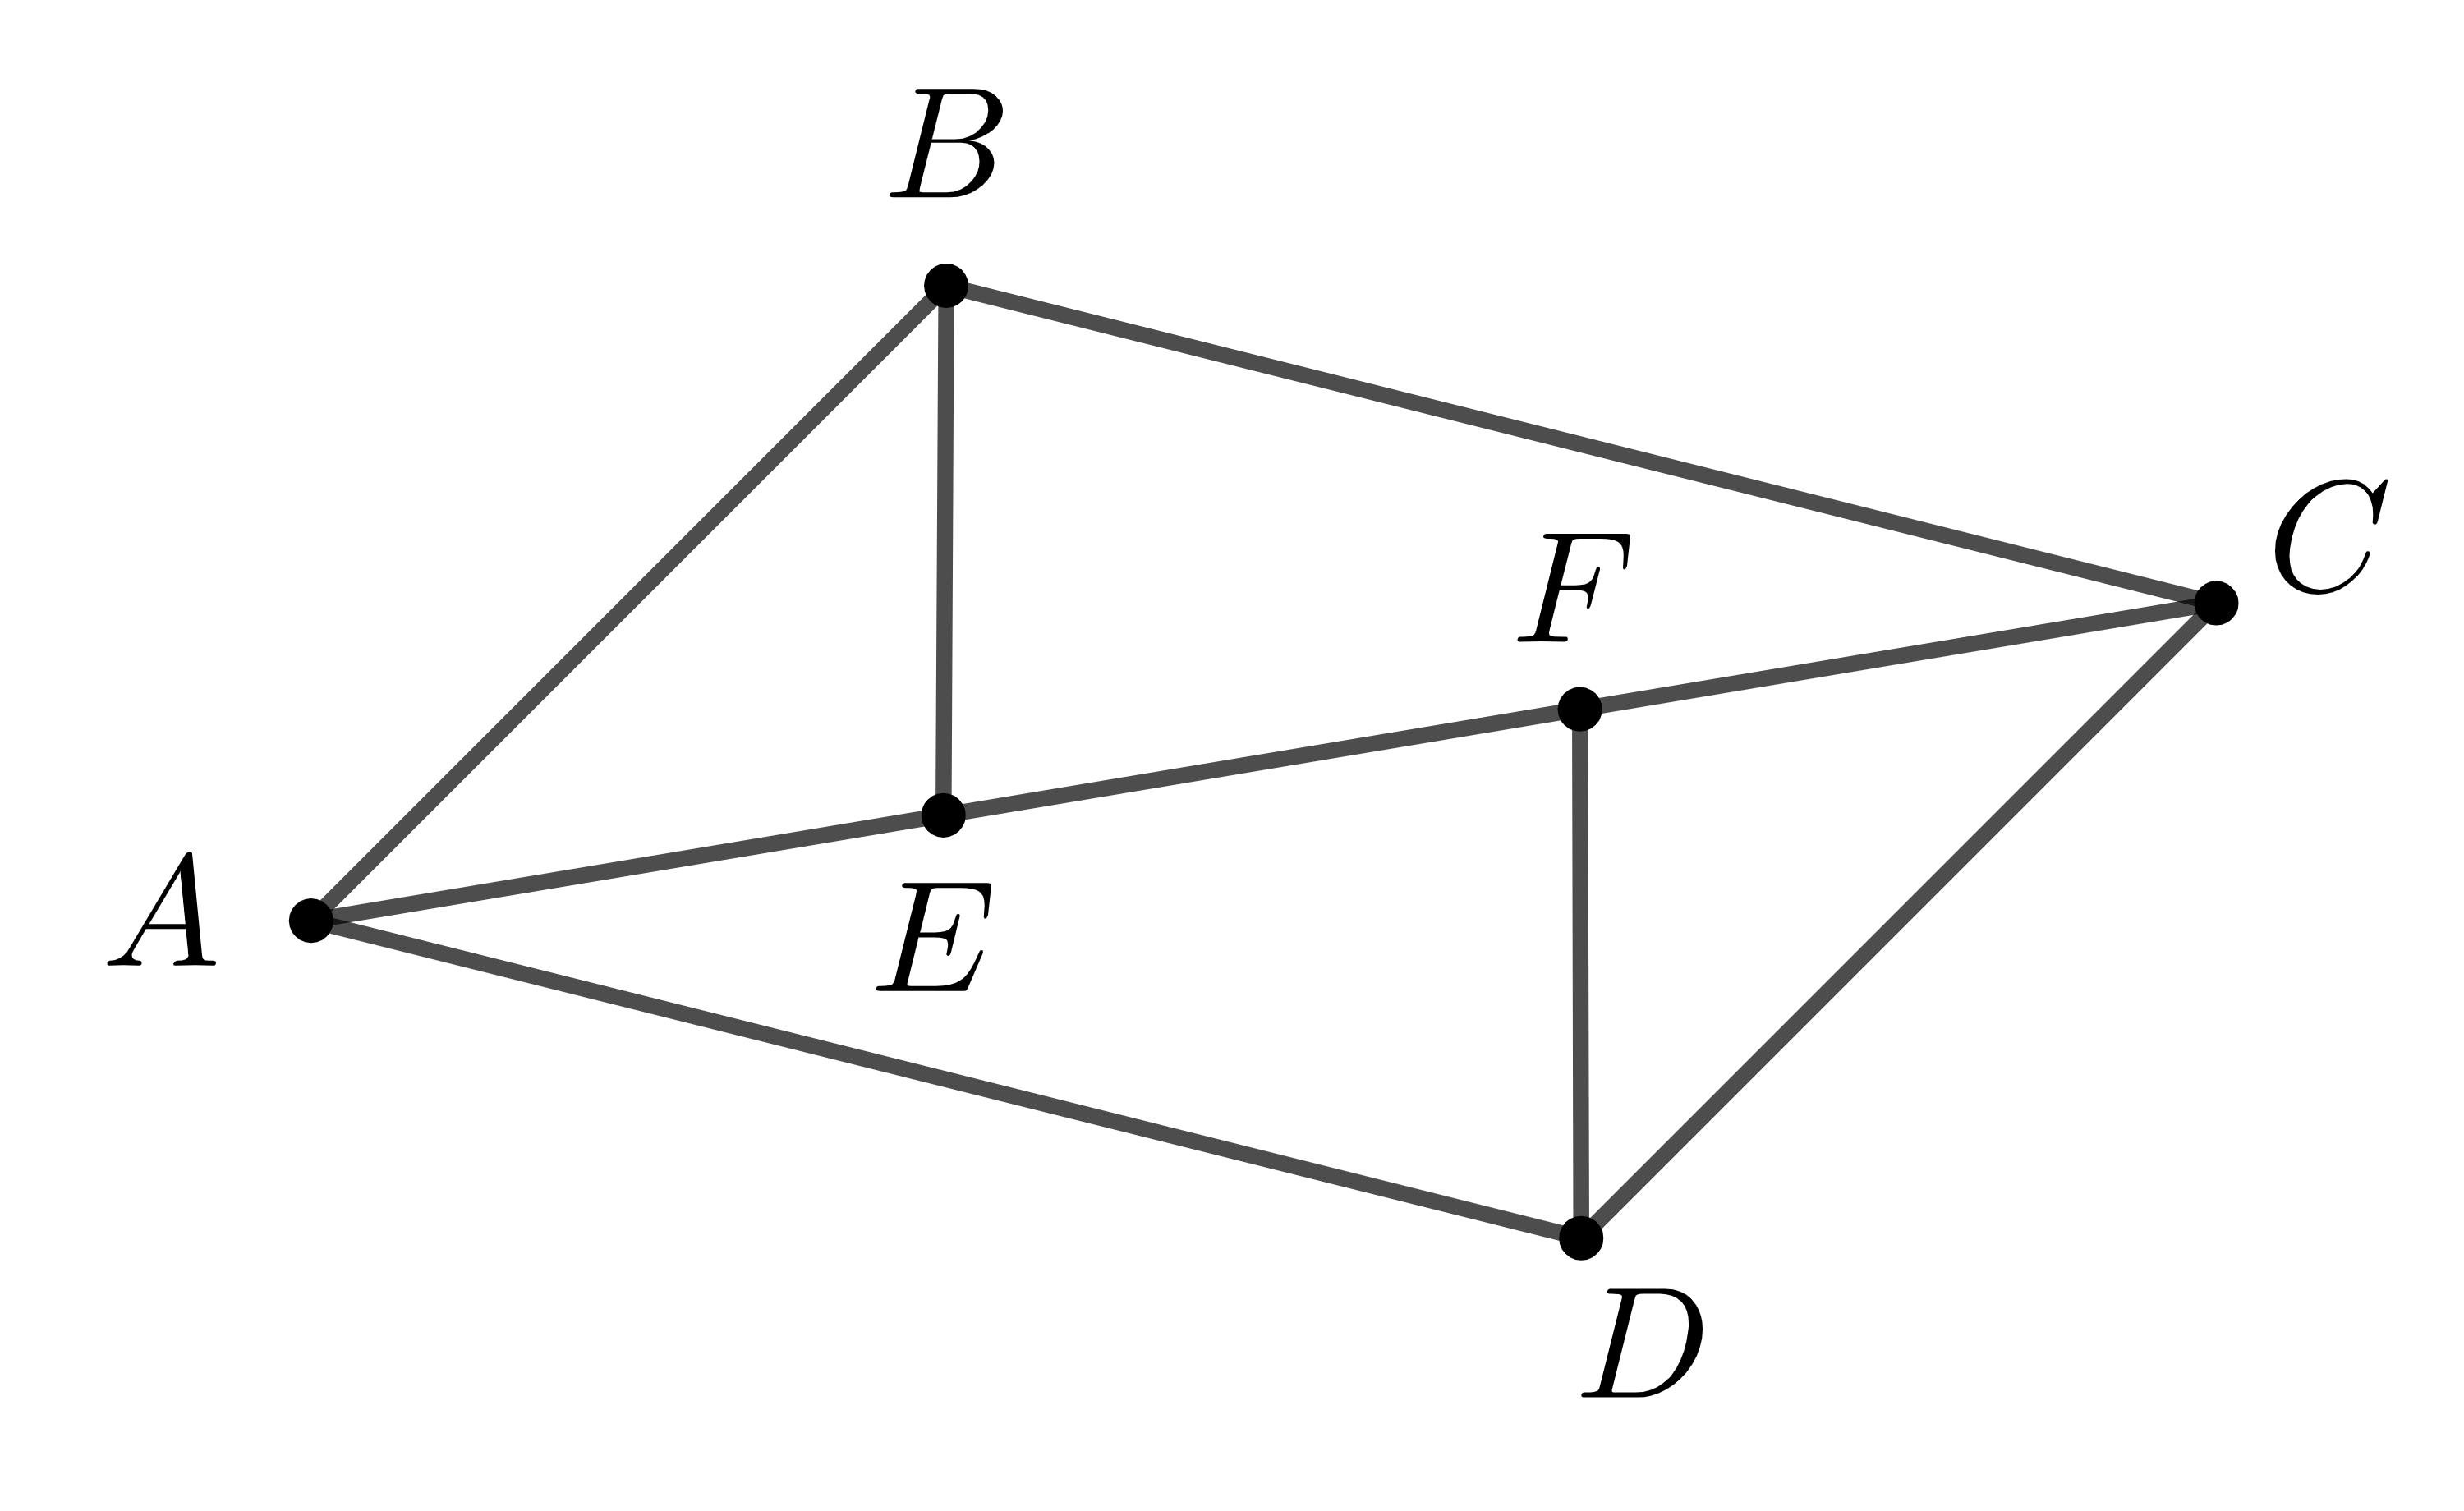
\includegraphics[width=.3\textwidth]{20260404/pics/20260404_inzh_1.png}
\end{problem}

\noindent\grid{34}{18}

\begin{center}
\textbf{Дополнительные задачи}
\end{center}

\samerowans{\begin{problem}{11}
Две высоты равнобедренного треугольника, проведённые к боковой стороне и основанию, пересекаются под углом $110°$. Найдите углы треугольника.
\end{problem}}

\smallskip

\samerowans{\begin{problem}{12}
Какое число надо прибавить к многочлену $9x^2 + 30x - 3$, чтобы получить квадрат двучлена?
\end{problem}}

\smallskip

\begin{problem}{13}
Докажите, что разность квадратов двух последовательных натуральных чисел есть число нечётное.
\end{problem}

\smallskip

\noindent\grid{34}{18}
```